\documentclass[11pt,a4paper]{article}

\usepackage[utf8]{inputenc}
\usepackage[T1]{fontenc}
\usepackage[margin=2.4cm]{geometry}
\usepackage{amsmath,amssymb}
\usepackage{amsthm}
\theoremstyle{definition}
\newtheorem{definition}{Definition}
\usepackage{booktabs}
\usepackage{array}
\usepackage{enumitem}
\usepackage{xcolor}
\usepackage{graphicx}
\usepackage{tikz}
\usetikzlibrary{arrows.meta,positioning,fit,backgrounds,calc}
\usepackage{hyperref}
\hypersetup{colorlinks=true,linkcolor=black,citecolor=black,urlcolor=blue!50!black}

\setlength{\parskip}{5pt}
\setlength{\parindent}{0pt}

\title{Experimentation protocol (working draft)\\[2pt]
\large Unsupervised structural clustering of the eukaryotic virome}
\author{Pascal Nardi --- M2 internship}
\date{\today}

\begin{document}
\maketitle

\tableofcontents
\vspace{4pt}
\hrule

\section{General idea}

Viral proteins change in sequence much faster than they change in shape. Because
of that, the usual sequence-based homology searches miss real relationships that
are still visible at the level of the 3D fold. The idea behind DeltaFold is to
learn, without labels, an embedding space where two viral proteins end up close
together when they share a fold, so that clustering the embeddings recovers known
protein families and possibly suggests structural links that sequence methods
cannot find.

So the biological question I would like the method to be able to answer is
whether an unsupervised structural encoder can recover viral protein families,
and whether it can connect families that have diverged in sequence but are still
structurally related. The methodological question I would like your opinion on is
whether the setup below is enough to tell apart real structural learning from the
model just exploiting easy shortcuts or collapsing its representation.

\section{Dataset}

\subsection{Source}

I use the predicted structural proteome of the eukaryotic virome from Nomburg et
al.~\cite{nomburg2024}. The release has 67,715 predicted protein structures
across 4,463 eukaryotic viral species. The structures are organised by family on
disk, which gives me weak family labels. I only use those labels to evaluate the
model, never during training.

\subsection{Quality filtering}

Each structure is a prediction, so confidence varies a lot. I read the
per-residue pLDDT from the B-factor column of each structure and drop any protein
whose mean pLDDT is below 70, which I found to be the usual cut for a confident
prediction. I also leave out the proteins with no assigned family when building
the labelled evaluation set. After filtering, around 67,000 proteins remain.

\subsection{How each protein is represented}

Before training, I convert every protein into a Protein Combinatorial Complex,
the multi-rank topological structure introduced for protein representation
learning by Topotein~\cite{topotein}. It organises a protein at four ranks:

\begin{itemize}[leftmargin=1.4em,itemsep=2pt]
  \item Rank 0, the residues, treated as nodes.
  \item Rank 1, the interactions, treated as edges.
  \item Rank 2, the secondary-structure elements (helices, strands, loops).
  \item Rank 3, the whole protein, as a single global node.
\end{itemize}

The four ranks instantiate, for proteins, the Protein Combinatorial Complex of
Topotein; the rank-1, rank-2 and rank-3 cells are constructed as follows, and the
full per-protein construction (the lifting pipeline) is detailed in
Section~\ref{sec:lifting}.

\paragraph{Rank-1 cells (interactions).} In the Protein Combinatorial Complex the
rank-1 cells are the interactions between residues. The motivation for building
them geometrically, rather than from the sequence, is that the fold is determined
by which residues are physically in contact in 3D, and two residues that are far
apart along the chain can be neighbours in space. I therefore instantiate the
interactions as a spatial graph: I take the C$\alpha$ atom as the position of each
residue, compute all pairwise C$\alpha$--C$\alpha$ distances, and connect each
residue to its 16 nearest neighbours in space (the residue itself is at distance
zero and is excluded). This gives a directed $k$-nearest-neighbour graph with
$k=16$. The choice of a $k$-NN contact graph over C$\alpha$ atoms is my
implementation of the rank-1 interactions; it is the standard way of turning a
structure into a contact graph, and it keeps the number of edges linear in the
number of residues.

A rank-1 cell joining a source residue $i$ to a neighbour $j$ carries three
pieces of geometric information: the scalar distance $d_{ij}=\lVert c_i-c_j\rVert$
between their C$\alpha$ atoms; a sinusoidal (Fourier) encoding of that single
scalar into a 16-dimensional vector, using the same sine/cosine scheme as a
positional encoding but applied to the distance value, which gives the network a
smooth multi-scale representation of $d_{ij}$; and the displacement vector
$c_j-c_i\in\mathbb{R}^3$. The scalar model used here feeds the attention layers
the distance and its 16-dimensional encoding (17 numbers); the displacement
vector is stored in the complex but not consumed by the present scalar model,
and is kept for a future geometric (vector-feature) variant.

\paragraph{Rank-2 cells (secondary-structure elements).} These are built in three
steps. First, every residue is assigned a secondary-structure state from the 3D
coordinates using a DSSP-style annotation, reduced to three classes: helix,
strand, and coil/loop. Second, consecutive residues that share the same state are
grouped into one contiguous segment, so each helix, each strand and each loop
becomes a single rank-2 cell. Third, the shape of each segment is summarised by a
principal-component analysis of its C$\alpha$ coordinates; the precise
construction (covariance matrix, eigenvalues, and the five shape descriptors) is
given in Section~\ref{sec:lifting}. Together with a one-hot encoding of the
segment type, this yields the 12 features that describe each secondary-structure
element, and the residue-to-segment membership is stored so the model knows which
residues compose each element.

\subsection{The lifting pipeline}
\label{sec:lifting}

Lifting is the offline step that turns a predicted structure (a PDB file) into the
Protein Combinatorial Complex described above. It runs once per protein, before
any training, and proceeds as follows.

\paragraph{Backbone and structural alphabet.} I read the atomic structure and keep
the C$\alpha$ trace $c_1,\dots,c_n\in\mathbb{R}^3$ of the first chain. From the
backbone I compute the dihedral angles $(\phi_i,\psi_i)$ of each residue, encoded
as $(\sin\phi_i,\cos\phi_i,\sin\psi_i,\cos\psi_i)$ so that the angle wraps
smoothly. In parallel I run Foldseek~\cite{foldseek} on the structure to obtain
its 3Di sequence, the structural-alphabet token of each residue. The 3Di alphabet
is a 20-letter code in which each letter summarises the local tertiary
environment of a residue (its orientation relative to its spatial neighbours), so
it is a structural, not a sequence, descriptor.

\paragraph{Rank-0 features: 3Di, not amino acid.} To make this explicit: each
residue (rank-0 cell) is described by its 3Di token, one-hot encoded, together
with the four dihedral numbers above. The amino-acid identity is extracted by the
pipeline but is deliberately not used, so the rank-0 features are purely
structural. This is a design choice: I want the encoder to rely on the geometry
of the fold rather than on residue composition.

\paragraph{Rank-1 cells.} The contact graph is built as in Section~2.3: a directed
$16$-nearest-neighbour graph over the C$\alpha$ atoms, each edge carrying the
distance $d_{ij}$, its 16-dimensional sinusoidal encoding, and the displacement
vector $c_j-c_i$.

\paragraph{Rank-2 and rank-3 shape descriptors.} A set of C$\alpha$ points (the
residues of one secondary-structure segment for rank 2, or the whole protein for
rank 3) is summarised by a principal-component analysis of its spatial spread.
For points $c_1,\dots,c_m$ with centroid $\bar c=\frac1m\sum_i c_i$, form the
$3\times 3$ covariance matrix
\[
\Sigma=\frac{1}{m-1}\sum_{i=1}^{m}(c_i-\bar c)(c_i-\bar c)^{\top},
\qquad
\Sigma=\sum_{a=1}^{3}\lambda_a\,u_a u_a^{\top},\quad \lambda_1\ge\lambda_2\ge\lambda_3\ge 0,
\]
where the eigenvalues $\lambda_1,\lambda_2,\lambda_3$ measure how extended the set
is along its three principal axes. From them I form five scale-normalised shape
descriptors, standard in point-cloud geometry,
\[
\begin{aligned}
&\text{linearity}=\frac{\lambda_1-\lambda_2}{\lambda_1},\quad
\text{planarity}=\frac{2(\lambda_2-\lambda_3)}{\lambda_1+\lambda_2},\quad
\text{scattering}=\frac{3\lambda_3}{\lambda_1+\lambda_2+\lambda_3},\\[2pt]
&\text{omnivariance}=\operatorname{sign}(\lambda_1\lambda_2\lambda_3)\,
|\lambda_1\lambda_2\lambda_3|^{1/3},\quad
\text{anisotropy}=\frac{\lambda_1-\lambda_3}{\lambda_1}.
\end{aligned}
\]
A rank-2 cell stores its type one-hot (helix / strand / loop, with a catch-all
slot), these five descriptors, and the three eigenvalues, for 12 features in
total. The rank-3 cell stores the protein size $n$, its radius of gyration
$R_g=\sqrt{\tfrac1n\sum_i\lVert c_i-\bar c\rVert^2}$, and the same five shape
descriptors and three eigenvalues computed over the whole C$\alpha$ trace, for 10
features in total. All of these quantities are functions of interatomic distances
only, so they are unchanged by any rotation or translation of the protein
(Section~\ref{sec:pccnn} returns to this invariance).

\subsection{Train / validation split}

The runs use a phylogenetic split: proteins are partitioned by taxonomic id so
that the train and validation sets contain different viral taxa. The point is to
stop the model from passing validation just by memorising taxon-level
regularities.

One thing I want to raise: a phylogenetic split removes taxonomic leakage but not
structural leakage. Two unrelated taxa can still share a fold, so some validation
proteins will have a structural near-twin in the training set. I think this is
acceptable because it reflects reality, but it means the validation numbers tell
me ``can the encoder place a known fold in the right place'', not ``can it
generalise to a fold it has never seen''. If we want the second claim, I would
need to also hold out a set of folds entirely.

\section{Topological deep learning: from CNNs to CCNNs}

This section gives the theoretical background that the architecture rests on. The
goal is to explain why a topological model is a natural choice for protein
structure, by following the line CNN $\to$ GNN $\to$ CCNN in which each step lifts
a limitation of the previous one, and to make precise the notion of equivariance
that organises this progression.

\subsection{Equivariance and invariance}

Let a group $G$ act on an input space $\mathcal{X}$ and on an output space
$\mathcal{Y}$. A map $f:\mathcal{X}\to\mathcal{Y}$ is $G$-equivariant if
\[
 f(g\cdot x)=g\cdot f(x)\qquad\text{for all }g\in G,\ x\in\mathcal{X},
\]
and $G$-invariant if $f(g\cdot x)=f(x)$ for all $g,x$, the special case where $G$
acts trivially on the output. Equivariance encodes a symmetry that the problem is
known to have, so that the model does not need to learn it from data. The three
families below are each defined by the symmetry group they respect, and each
enlarges the domain on which the model can act.

\subsection{Convolutional networks: grids and translation}

A convolutional network acts on data supported on a regular grid (image pixels,
audio samples). A convolutional layer slides one small filter across all
positions; sharing the filter makes the layer equivariant to the translation
group, that is, shifting the input shifts the output by the same amount. Weight
sharing also gives locality and a parameter count independent of the input size.
The limitation is that a grid is a rigid domain with a fixed neighbourhood and a
global coordinate system, so CNNs do not apply to data whose elements have no
canonical ordering or position, such as the residues of a protein whose contacts
are irregular.

\subsection{Graph neural networks: graphs and permutation}

Graph neural networks remove the grid assumption. The data live on a graph
$G=(V,E)$ and a layer updates each vertex from its neighbours by message
passing~\cite{mpnn}:
\[
 h_v'=\beta\!\Big(h_v,\ \textstyle\bigoplus_{u\in\mathcal{N}(v)}\alpha(h_v,h_u)\Big),
\]
where $\bigoplus$ is a permutation-invariant aggregation (sum, mean, or max).
Because the aggregation ignores the order of the neighbours, a GNN is equivariant
to permutations of the vertices: relabelling the nodes relabels the outputs the
same way, which is the right symmetry for objects with no canonical node order.
The limitation that motivates the next step is that a graph only encodes binary
relations: an edge joins exactly two vertices. A protein, however, has natural
higher-order parts, a whole $\alpha$-helix, a $\beta$-sheet, the entire chain,
that are relations among many residues at once, and a plain graph has no
first-class object for them. Reaching distant residues also requires stacking
many layers, which tends to oversquash information through bottlenecks.

\subsection{Combinatorial complex networks: higher-order and hierarchical relations}

Combinatorial complex neural networks~\cite{hoan} keep permutation equivariance
but replace the graph by a combinatorial complex, a domain with cells of several
ranks: rank-0 cells are the vertices, rank-1 cells the edges, and higher-rank
cells are groups of vertices treated as single objects, ordered by a rank that
encodes a hierarchy. Message passing then happens not only between vertices but
between cells of different ranks, so a helix (a rank-2 cell) can send and receive
messages as a unit. This addresses both GNN limitations at once: higher-order
parts become explicit objects, and a message between a residue and the helix it
belongs to is a single step rather than a long chain of vertex-to-vertex hops.
The next section makes combinatorial complexes and their message passing precise.

\section{Combinatorial complexes and CCNNs}
\label{sec:ccnn}

\subsection{Combinatorial complexes}

\begin{definition}[Combinatorial complex, Hajij et al.~\cite{hoan}]
A combinatorial complex is a triple $(S,\mathcal{X},\mathrm{rk})$ where $S$ is a
finite set of entities, $\mathcal{X}\subseteq\mathcal{P}(S)\setminus\{\emptyset\}$
is a set of cells, and $\mathrm{rk}:\mathcal{X}\to\mathbb{Z}_{\ge 0}$ is a rank
function such that (i) $\{s\}\in\mathcal{X}$ for every $s\in S$, and (ii)
$\mathrm{rk}$ is monotone, $x\subseteq y\Rightarrow\mathrm{rk}(x)\le\mathrm{rk}(y)$.
\end{definition}

A cell $x$ with $\mathrm{rk}(x)=k$ is a $k$-cell, and $\mathcal{X}^k$ is the set of
$k$-cells. Two familiar domains are special cases: a graph is the complex whose
only cells are singletons and pairs with ranks 0 and 1, and a simplicial or cell
complex is the case where cells are closed under taking subsets (faces). A
combinatorial complex keeps the hierarchy (the rank) of the latter while allowing
arbitrary set-type cells like the former, which is exactly what is needed to host
residues, contacts, secondary-structure elements and the whole protein inside one
object.

\subsection{Neighborhood functions}

The structure of a complex is carried by two kinds of neighbourhood relation
between cells. Two cells are incident when one contains the other ($x\subseteq y$
or $y\subseteq x$); incidence links cells of different ranks, for instance a
residue and the helix that contains it. Two cells of the same rank are adjacent
when they are both contained in a common higher-rank cell (or both contain a
common lower-rank cell). Each relation is stored as a neighbourhood matrix; in
particular the incidence matrix $B_{r,k}\in\{0,1\}^{|\mathcal{X}^r|\times|\mathcal{X}^k|}$
has a $1$ in entry $(x,y)$ when the $r$-cell $x$ is incident to the $k$-cell $y$.
These matrices are the discrete operators that move information between ranks.

\subsection{Cochains and higher-order message passing}

Features live on cells. A rank-$k$ cochain is a matrix
$H_k\in\mathbb{R}^{|\mathcal{X}^k|\times d_k}$ whose rows are the feature vectors
of the $k$-cells. A CCNN layer updates these cochains by higher-order message
passing. For a target cell $x$, a chosen neighbourhood function $\mathcal{N}$ and
neighbours $y\in\mathcal{N}(x)$,
\[
 m_{y\to x}=\alpha\!\left(h_x,h_y\right),\qquad
 m_x^{\mathcal{N}}=\bigoplus_{y\in\mathcal{N}(x)}m_{y\to x},\qquad
 h_x'=\beta\!\Big(h_x,\ \bigoplus_{\mathcal{N}}m_x^{\mathcal{N}}\Big),
\]
where $\alpha$ builds a message from a neighbour, $\bigoplus$ is a
permutation-invariant aggregation, and $\beta$ updates the cell. In an attention
CCNN the message $\alpha(h_x,h_y)$ is a learned weight times a transformed value
of $h_y$, with the weights normalised over $\mathcal{N}(x)$; this is exactly the
attention mechanism the model uses, with the neighbourhoods given by the
incidence matrices of the complex.

\subsection{Permutation equivariance}

Let $P_k$ be a permutation matrix that relabels the $k$-cells. If every cochain is
relabelled, $H_k\mapsto P_kH_k$, and every incidence matrix accordingly,
$B_{r,k}\mapsto P_rB_{r,k}P_k^{\top}$, then a CCNN layer commutes with the
relabelling, and its output transforms as $H_k'\mapsto P_kH_k'$. CCNNs are
therefore permutation-equivariant, the higher-order analogue of the permutation
equivariance of GNNs. A protein-level prediction is made permutation-invariant by
ending with a symmetric pooling over cells.

\section{The Protein Combinatorial Complex and attention}
\label{sec:pccnn}

Topotein~\cite{topotein} instantiates this framework for proteins. The Protein
Combinatorial Complex (PCC) is a combinatorial complex with four ranks: rank-0
residues, rank-1 interactions (the spatial contacts of Section~2.3), rank-2
secondary-structure elements, and a single rank-3 cell for the whole protein. Its
incidence matrices record which residues form each contact ($B_{0,1}$), which
residues compose each secondary-structure element ($B_{0,2}$), and that every cell
belongs to the one protein cell ($B_{0,3}$, $B_{2,3}$). Topotein's network,
TCPNet, performs attention-based higher-order message passing across these ranks
and is SE(3)-equivariant: it carries geometric vector features next to scalar
ones, so that rotating or translating the protein rotates or translates the vector
features consistently.

The present model uses the same PCC domain and the same attention-based message
passing across ranks, but takes a simpler route to geometric symmetry. Rather than
carrying equivariant vector channels, it describes every cell by quantities that
are already invariant to rigid motions, namely interatomic distances, backbone
dihedral angles, and the eigenvalue-based shape descriptors of
Section~\ref{sec:lifting}. Because these inputs are unchanged by any rotation or
translation of the protein, and the message passing only combines them with
permutation-invariant aggregations, the resulting protein embedding is
SE(3)-invariant by construction and permutation-invariant after the final
pooling. This is the property wanted for clustering: two copies of the same fold
placed differently in space must receive the same embedding.

\section{Architecture}

The model is a higher-order attention network (an attention CCNN in the sense of
Section~\ref{sec:ccnn}) that operates directly on the Protein Combinatorial Complex, following
Topotein~\cite{topotein,hoan}. It passes messages between the ranks of the complex
(residues, edges, secondary structure, whole protein) and not only between
residues.

\subsection{Features per rank}

The residue nodes are described by purely structural and geometric features: the
3Di structural-alphabet token from Foldseek~\cite{foldseek} and the backbone
dihedral angles. I deliberately leave out amino-acid identity and any
sequence-order information, so the model has to rely on the geometry of the fold
rather than on composition or position along the chain. The features that are
actually used are:

\begin{center}
\begin{tabular}{@{}l l l@{}}
\toprule
Rank & Entity & Features used\\
\midrule
0 & Residue   & 3Di structural-alphabet token, backbone dihedrals $(\phi,\psi)$\\
1 & Edge      & C$\alpha$--C$\alpha$ distance, sinusoidal distance encoding, displacement vector\\
2 & SSE       & type (helix/strand/loop), 5 shape descriptors, 3 covariance eigenvalues (12 dims)\\
3 & Protein   & size, radius of gyration, 5 shape descriptors, 3 gyration eigenvalues (10 dims)\\
\bottomrule
\end{tabular}
\end{center}

Each rank is mapped to a common width of 128 by a small two-layer perceptron
before the attention layers.

\subsection{The attention layer}
\label{sec:attention}

The core operation of the model is attention, so it is worth saying plainly what
that means before writing it formally. Attention lets one element build an updated
description of itself by taking a weighted average of information coming from a set
of other elements, where the model itself decides how much weight each neighbour
gets. The element being updated emits a query vector $q$, every candidate
neighbour emits a key $k$ and a value $v$, and the weight given to a neighbour is
large when its key matches the query and small otherwise. The updated element is
the weighted sum of the neighbours' values. The weights are not fixed in advance,
so a residue can learn to attend to the residues that matter for its local fold
rather than to a fixed window of sequence neighbours.

\paragraph{Message passing on the complex.} Each step of a layer is one instance
of the higher-order message passing of Section~\ref{sec:ccnn}, applied along one
incidence relation of the Protein Combinatorial Complex. Writing $h_x$ for the
current feature of cell $x$, and $W_q,W_k,W_v$ for learned projections, the
message from a neighbour $y$ to a cell $x$ and the update of $x$ are
\[
 e_{xy}=\frac{(W_q h_x)^{\top}(W_k h_y)}{\sqrt{d}}-\gamma\,d_{xy},\qquad
 a_{xy}=\frac{\exp(e_{xy})}{\sum_{y'\in\mathcal{N}(x)}\exp(e_{xy'})},\qquad
 h_x'=\mathrm{LN}\!\Big(h_x+\textstyle\sum_{y\in\mathcal{N}(x)}a_{xy}\,W_v h_y\Big),
\]
where $d$ is the feature width, $\mathcal{N}(x)$ is the neighbourhood given by the
relevant incidence matrix, $\mathrm{LN}$ is layer normalisation (so the update is a
residual), and $-\gamma\,d_{xy}$ is a small geometric bias ($\gamma$ small,
fixed) that, where a C$\alpha$--C$\alpha$ distance $d_{xy}$ is defined, gives more
weight to spatially closer neighbours. The softmax normalisation over
$\mathcal{N}(x)$ is the permutation-invariant aggregation of the message-passing
scheme.

\paragraph{The four steps and their topology.} The network stacks four identical
layers, and within each layer attention is applied four times, once per incidence
relation of the complex:

\begin{enumerate}[leftmargin=1.6em,itemsep=3pt]
  \item Residues $\to$ edges, along $B_{0,1}$: each edge attends to its source
        residue and updates its own description, summarising the local environment
        of that residue.
  \item Residues $\to$ secondary-structure elements, along $B_{0,2}$: each
        element attends over the residues that compose it (its column of
        $B_{0,2}$), so a helix or strand gathers information from its constituent
        residues.
  \item Edges $\to$ residues, along $B_{0,1}^{\top}$: each residue attends over
        the edges arriving at it and is refined; this is where a residue
        integrates its spatial neighbourhood.
  \item Residues and elements $\to$ whole protein, along $B_{0,3}$ and $B_{2,3}$:
        the residue and element features are mean-pooled and used to update the
        single rank-3 cell.
\end{enumerate}

Each of the four updates is a residual followed by layer normalisation, which
keeps training stable. The first three steps move information up and down the
incidence relations between ranks 0, 1 and 2; the fourth pools into the rank-3
cell, which is what lets a global summary of the protein build up across layers.

\paragraph{Readout.} After the four layers, the final protein embedding is
produced by mean-pooling the residue features, concatenating the result with the
rank-3 cell, passing it through a last perceptron, and $\ell_2$-normalising it, so
that every protein becomes a point on the unit sphere. The mean-pool makes the
embedding permutation-invariant, and the invariant input features make it
SE(3)-invariant (Section~\ref{sec:pccnn}). Distances on the sphere are what I
later cluster.

\subsection{Schematic of the model}

Figure~\ref{fig:tensor} draws one layer as a tensor diagram in the convention of
Hajij et al.~\cite{hoan}: the nodes are the cochain spaces $C^{r}$ (the feature
arrays of the rank-$r$ cells), and each directed arrow is a cochain map given by
an incidence matrix $B_{r,k}$ of the complex, that is, one attention step from
rank $r$ to rank $k$. When two maps feed the same target they meet at a merge node
(the solid dot), where their messages are aggregated before the target is updated;
here this is how the residue and element cochains are pooled into the single
rank-3 protein cell. The block is applied four times, and a final readout turns the
residue and protein cochains into the embedding $z$.

\begin{figure}[h]
\centering
\resizebox{0.95\textwidth}{!}{%
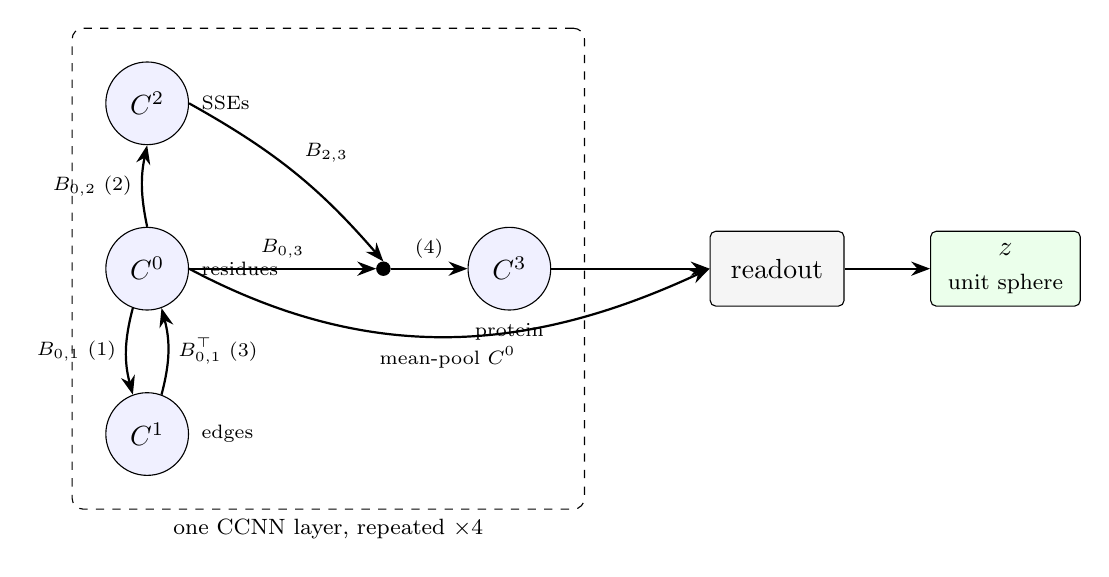
\begin{tikzpicture}[
  >={Stealth[length=2.4mm]},
  cc/.style={circle, draw, minimum size=1.05cm, align=center, fill=blue!6},
  merge/.style={circle, draw, fill=black, inner sep=1.7pt},
  head/.style={draw, rounded corners=2pt, minimum width=1.7cm, minimum height=0.95cm, align=center, fill=gray!8},
  emb/.style={draw, rounded corners=2pt, minimum width=1.9cm, minimum height=0.95cm, align=center, fill=green!8},
  wire/.style={->, thick}
]
% cochain-space nodes
\node[cc] (c2) at (0,2.1)  {$C^{2}$};
\node[cc] (c0) at (0,0)    {$C^{0}$};
\node[cc] (c1) at (0,-2.1) {$C^{1}$};
\node[merge] (m) at (3.0,0) {};
\node[cc] (c3) at (4.6,0)  {$C^{3}$};

% rank labels
\node[font=\scriptsize,right=1pt of c2] {SSEs};
\node[font=\scriptsize,right=1pt of c0] {residues};
\node[font=\scriptsize,right=1pt of c1] {edges};
\node[font=\scriptsize,below=1pt of c3] {protein};

% cochain maps (incidence matrices) as labelled arrows
\draw[wire] (c0.250) to[bend right=15] node[left,font=\scriptsize]{$B_{0,1}$ (1)} (c1.110);
\draw[wire] (c1.70)  to[bend right=15] node[right,font=\scriptsize]{$B_{0,1}^{\top}$ (3)} (c0.290);
\draw[wire] (c0.north) to[bend left=12] node[left,font=\scriptsize]{$B_{0,2}$ (2)} (c2.south);
\draw[wire] (c0.east) -- node[above,font=\scriptsize]{$B_{0,3}$} (m.west);
\draw[wire] (c2.east) to[bend left=10] node[above right,font=\scriptsize]{$B_{2,3}$} (m.north);
\draw[wire] (m.east) -- node[above,font=\scriptsize]{(4)} (c3.west);

% layer box
\begin{scope}[on background layer]
\node[draw,dashed,rounded corners,fit=(c2)(c1)(c3),inner sep=12pt,
      label=below:{\footnotesize one CCNN layer, repeated $\times 4$}] (layer) {};
\end{scope}

% readout
\node[head] (head) at (8.0,0) {readout};
\node[emb]  (z)    at (10.9,0) {$z$\\ \footnotesize unit sphere};
\draw[wire] (c3.east) -- (head.west);
\draw[wire] (c0.east) to[out=-28,in=205] node[below,font=\scriptsize]{mean-pool $C^{0}$} (head.west);
\draw[wire] (head.east) -- (z.west);
\end{tikzpicture}%
}
\caption{One layer of the model as a tensor diagram in the convention of
Hajij et al.~\cite{hoan}. Nodes are the cochain spaces $C^{0}\!-\!C^{3}$
(residues, edges, SSEs, whole protein); each arrow is a cochain map given by an
incidence matrix of the Protein Combinatorial Complex, i.e.\ one attention step.
The numbered steps are: (1) residues$\to$edges along $B_{0,1}$, (2)
residues$\to$SSEs along $B_{0,2}$, (3) edges$\to$residues along $B_{0,1}^{\top}$,
(4) pooling residues and SSEs into the protein cell along $B_{0,3}$ and $B_{2,3}$,
which meet at the merge node (solid dot). The block is applied four times; a
readout then mean-pools $C^{0}$, combines it with $C^{3}$, and $\ell_2$-normalises
the result into the embedding $z$.}
\label{fig:tensor}
\end{figure}

\subsection{Hyperparameters}

\begin{center}
\begin{tabular}{@{}l l l@{}}
\toprule
Group & Hyperparameter & Value\\
\midrule
Model & embedding width        & 128\\
      & attention layers       & 4\\
      & dropout                & 0.1\\
      & graph degree $k$       & 16\\
      & output dim             & 128, $\ell_2$-normalised\\
\midrule
Optim & optimizer              & AdamW\\
      & learning rate          & $1\times10^{-4}$\\
      & weight decay           & $1\times10^{-5}$\\
      & scheduler              & reduce-on-plateau (factor 0.5, patience 2)\\
      & gradient clip          & value clip 1.0\\
      & epochs                 & 50\\
      & batch size             & 64 proteins\\
      & residue budget / batch & 3500\\
\midrule
Loss  & contrastive temperature $\tau$ & 0.1\\
      & TM-score auxiliary weight       & 0.1\\
\bottomrule
\end{tabular}
\end{center}

\section{Training method}

\subsection{What contrastive learning is}

The model is trained without any family labels, using contrastive learning. The
principle is simple: I take each protein and make two slightly perturbed copies of
it, then I train the encoder so that the two copies of the same protein land close
together in the embedding space while copies of different proteins are pushed
apart. Over many proteins, the only way to satisfy this everywhere is to place
proteins that are genuinely alike near each other and proteins that differ far
apart. The encoder therefore discovers, on its own, the features that make two
proteins similar, without ever being told what the families are.

There are two useful ways to read this objective. First, in information terms, the
two perturbed copies are two ``views'' of the same underlying structure, and the
contrastive loss is a lower bound on the mutual information between the embeddings
of the two views~\cite{infonce}: maximising it forces the embedding to keep
exactly what is common to both views (the fold) and to discard what the
perturbation changed (the noise). Second, on the unit sphere the loss splits into
two competing forces~\cite{alignunif}: an alignment force that pulls the two views
of one protein together, and a uniformity force, carried by the negatives, that
spreads all proteins out over the sphere. Without negatives the alignment force
alone is minimised by mapping every protein to the same point, which is the
representational collapse the health checks of Section~\ref{sec:health} are meant
to catch; the negatives are what keep the embedding spread out and informative.

\subsection{SimCLR and the two views}

The exact recipe I follow is SimCLR~\cite{simclr}, a standard contrastive
framework. For each protein I generate two augmented ``views'' of its complex.
The augmentations are meant to act like measurement noise rather than to change
the fold: I add small Gaussian noise (about 0.3 to 0.5\,\AA) to the C$\alpha$
coordinates and recompute the local graph distances, and I randomly mask a
fraction of the residue features. The two views of one protein form a positive
pair that should be pulled together; every other protein in the batch provides
negative examples that should be pushed away.

\subsection{The NT-Xent (InfoNCE) loss}

The objective that turns this idea into a number to minimise is the NT-Xent loss,
the normalised temperature-scaled cross-entropy used in SimCLR, which is an
instance of the InfoNCE objective~\cite{infonce,simclr}. For a batch of $N$
proteins there are $2N$ views. Writing $z_i$ for the unit-length embedding of view
$i$, and $\mathrm{sim}(u,v)=u^{\top}v$ for the cosine similarity of two
unit-length vectors, the loss for a positive pair $(i,j)$ (the two views of the
same protein) is

\begin{equation*}
\ell_{i,j} \;=\; -\,\log
\frac{\exp\!\big(\mathrm{sim}(z_i,z_j)/\tau\big)}
     {\displaystyle\sum_{k=1}^{2N}\mathbf{1}_{[k\neq i]}\,
      \exp\!\big(\mathrm{sim}(z_i,z_k)/\tau\big)} ,
\end{equation*}

and the total loss is the average of $\ell_{i,j}$ over all positive pairs in the
batch. The numerator rewards the model for making the two views of the same
protein similar; the denominator penalises it for making a view similar to any
other protein in the batch. The temperature $\tau$ (set to 0.1) controls how
sharply the model focuses on the hardest negatives: a smaller $\tau$ makes the
loss pay more attention to negatives that are already close by.

\subsection{Hard-negative batches}

A contrastive model only learns something useful if the negatives are hard. If
the other proteins in a batch are obviously different, the model can tell them
apart using a cheap cue (for instance, just the protein length) and never has to
look at the fold. To prevent that, I build the batches deliberately: proteins are
binned by length and then ordered within a bin by their secondary-structure
composition, so each batch groups proteins that look superficially similar but
have a different topology. This forces the model to use the actual fold to
separate them. Batches are budgeted by total residue count rather than by a fixed
number of proteins, which keeps the per-step cost bounded on the 16\,GB machine.

\subsection{TM-score auxiliary term}

On top of the contrastive loss I add a small auxiliary term, weighted 0.1, that
regresses the true pairwise TM-score of sampled protein pairs (precomputed and
cached). TM-score is a standard measure of structural similarity between two
proteins, so this term ties the geometry of the embedding directly to a known
structural quantity, rather than letting it be shaped by the contrastive
objective alone.

\section{Plan of experiments}

\subsection{Metrics}

I evaluate the embeddings against the held-out family labels and against
ground-truth structural similarity. I report the adjusted Rand index of HDBSCAN
(density-based) clusters \cite{hdbscan} and TM-$\rho$ (the rank correlation
between embedding distance and pairwise TM-score).

The adjusted Rand index (ARI) compares the clustering of the embeddings to the
known families, corrected for what you would get by chance, on a scale where 0 is
random and 1 is perfect. It wobbles for two reasons. First, it depends on a
clustering step that is itself unstable: $k$-means starts from a random
initialisation, and HDBSCAN is density-based, so a small change in the embedding
can merge or split clusters and move the score by several points. Second, the
problem is hard and very imbalanced (around 2700 clusters with about 40\%
singletons), so the score reacts to a handful of borderline proteins changing
cluster. This is why the HDBSCAN ARI swings more than the $k$-means one: it is
the more sensitive of the two to small changes in the geometry.

TM-$\rho$ is different in kind: it is a rank correlation between distance in the
embedding and the TM-score (a standard measure of structural similarity) over a
sample of protein pairs. Because it does not involve any clustering, it is the
most stable of the two, sitting between about $-0.75$ and $-0.80$ across every
epoch. A negative value is what we want, since structurally similar proteins
(high TM-score) should end up close together (small distance). The small wobble
comes mostly from a different set of pairs being sampled each epoch rather than
from real changes in the model, and the fact that it barely moves suggests the
structural signal was picked up early and then stayed roughly constant.

The practical consequence is that no single epoch is a reliable readout. Reading
off epoch 20 alone would overstate things, because epoch 20 happens to be a local
high for the HDBSCAN ARI. A fairer summary is the level and trend over the last
several epochs, and ideally an average over a few random seeds. This is the main
reason I want the per-epoch health checks of Section~\ref{sec:health} and repeated runs before
drawing any conclusion from these numbers. 

\subsection{Baselines}

I want every number reported against two references on the same split: a random
or shuffled-embedding baseline as a floor, and Foldseek~\cite{foldseek} as the
method to beat. A result only means something relative to both.

\subsection{Health checks I want to run every epoch}
\label{sec:health}

Because a contrastive encoder can cheat by collapsing all embeddings toward a
common direction, I want to log a few diagnostics every epoch and treat them as
gating criteria rather than something I look at afterwards. These are the spread
of the embedding values per dimension (it should stay clearly above the collapse
threshold of about 0.02), the mean off-diagonal cosine similarity (it should stay
low; values near 0.9 to 0.97 mean the vectors are nearly parallel), and the
effective rank of the embedding covariance as a single number for how many
dimensions are actually being used. I would only interpret a checkpoint
biologically if these are healthy at that epoch.

\section{First results (preliminary)}

These numbers come from a single run on the 16\,GB machine. The training loss
converges very quickly: it falls from about 2.5 at the start of training to about
0.5 by the end of the first epoch, and after that it barely moves. The validation
loss behaves the same way, hovering around 0.40 for the rest of the run. In other
words the contrastive objective is essentially solved within the first epoch.

What is more interesting is that the evaluation metrics keep improving a little
even after the loss has flattened. Pushing the run from epoch 6 to epoch 20 still
buys a small but consistent gain in clustering quality: the HDBSCAN ARI rises from
about 0.25 to about 0.40, while TM-$\rho$ decreases (becomes more negative), which
means a stronger and therefore better anti-correlation between embedding distance
and structural similarity. So the embedding geometry is still being refined after
the loss plateaus, even though the gains are modest and noisy from epoch to
epoch. Table~\ref{tab:results} lists the values at the start of training, at
epoch 6, and at epoch 20.

The TM-$\rho$ column starts surprisingly negative ($-0.68$) even with completely
random weights, rather than near 0 as you might expect from an untrained model.
I checked this is not a bug (shuffling the embedding-to-protein correspondence
collapses it to $\approx 0$, as it should), so the correlation is real even
before any training happens. The likely explanation is that the model takes
the Foldseek 3Di structural alphabet as an input feature, and 3Di tokens are
themselves derived from local structure, so they are highly informative about
TM-score by construction; the early layers (linear $\to$ layer norm $\to$
SiLU $\to$ linear) are mostly information-preserving, so a random forward pass
still lets a lot of that structural signal leak straight through into the
embedding distances. Training then sharpens this further, from $-0.68$ to about
$-0.79$.

\begin{table}[h]
\centering
\begin{tabular}{@{}l c c c@{}}
\toprule
Metric & Initial & Epoch 6 & Epoch 20\\
\midrule
Training loss   & $\approx 2.5$ & 0.53    & 0.43\\
Validation loss & ---           & 0.41    & 0.38\\
ARI (HDBSCAN)   & 0.03          & 0.25    & 0.40\\
TM-$\rho$       & $-0.68$       & $-0.79$ & $-0.78$\\
\bottomrule
\end{tabular}
\caption{Preliminary results from a single run. ``Initial'' is a freshly
initialized model with random weights (no training), scored on the same
validation split as the later epochs; the validation loss is only recorded
from epoch 6 since random weights have no meaningful loss to report on that
scale. The training loss is essentially converged by epoch 6, yet the
clustering metrics continue to improve slightly through epoch 20, and both
clustering metrics show training pulls the embeddings well past the
random-weight baseline.}
\label{tab:results}
\end{table}

\begin{thebibliography}{9}

\bibitem{nomburg2024}
J. Nomburg, E. E. Doherty, N. Price, D. Bellieny-Rabelo, Y. K. Zhu, J. A. Doudna.
\newblock Birth of protein folds and functions in the virome.
\newblock \emph{Nature}, 633:710--717, 2024.
\newblock \url{https://doi.org/10.1038/s41586-024-07809-y}.

\bibitem{topotein}
Z. Wang, A. R. Jamasb, et al.
\newblock Topotein: Topological Deep Learning for Protein Representation Learning.
\newblock \emph{arXiv preprint} arXiv:2509.03885, 2025.

\bibitem{hoan}
M. Hajij, G. Zamzmi, T. Papamarkou, N. Miolane, A. Guzm\'an-S\'aenz,
K. N. Ramamurthy, T. Birdal, T. K. Dey, S. Mukherjee, S. N. Samaga, N. Livesay,
R. Walters, P. Rosen, M. T. Schaub.
\newblock Topological Deep Learning: Going Beyond Graph Data.
\newblock \emph{arXiv preprint} arXiv:2206.00606, 2022.

\bibitem{mpnn}
J. Gilmer, S. S. Schoenholz, P. F. Riley, O. Vinyals, G. E. Dahl.
\newblock Neural Message Passing for Quantum Chemistry.
\newblock \emph{Proceedings of ICML}, 2017. arXiv:1704.01212.

\bibitem{alignunif}
T. Wang, P. Isola.
\newblock Understanding Contrastive Representation Learning through Alignment and
Uniformity on the Hypersphere.
\newblock \emph{Proceedings of ICML}, 2020. arXiv:2005.10242.

\bibitem{simclr}
T. Chen, S. Kornblith, M. Norouzi, G. Hinton.
\newblock A Simple Framework for Contrastive Learning of Visual Representations
(SimCLR).
\newblock \emph{Proceedings of ICML}, 2020. arXiv:2002.05709.

\bibitem{infonce}
A. van den Oord, Y. Li, O. Vinyals.
\newblock Representation Learning with Contrastive Predictive Coding (InfoNCE).
\newblock \emph{arXiv preprint} arXiv:1807.03748, 2018.

\bibitem{foldseek}
M. van Kempen, S. S. Kim, C. Tumescheit, M. Mirdita, J. Lee, C. L. M. Gilchrist,
J. S\"oding, M. Steinegger.
\newblock Fast and accurate protein structure search with Foldseek.
\newblock \emph{Nature Biotechnology}, 42:243--246, 2024.

\bibitem{hdbscan}
R. J. G. B. Campello, D. Moulavi, J. Sander.
\newblock Density-Based Clustering Based on Hierarchical Density Estimates
(HDBSCAN).
\newblock \emph{Advances in Knowledge Discovery and Data Mining (PAKDD)}, 2013.

\end{thebibliography}

\end{document}
